\chapter{Implementation}

	\section{Prerequisites}
	\label{sec:prerequisitesimp}
	
	\subsection{Third-party services}
	\label{ssec:third-party-services}
	
	\ac{AWESOME}'s development relies on the use of a few third-party services in order to make development a little easier.
	By setting up these at the very start, valuable time and effort can be saved further down the project's lifecycle.
	
	TravisCI\footnote{TravisCI Homepage: \url{http://travis-ci.com}} was the first service I set up after receiving access to the GitHub repository.
	Travis allows for completely automated running of unit test suites whenever code is committed to Git.
	This is incredibly useful when working with modular libraries like the \ac{i18n} framework.
	Travis also allows for testing across PHP versions, so I could simultaneously test PHP 5.3, 5.4, 5.5, 5.6 and hhvm (a custom PHP server).
	
	\autoref{fig:travisbuild} shows when I made a change using a function that was new to PHP 5.6 that I wouldn't have noticed without Travis until a later date, as my development environment was running PHP 5.6.
	
	Travis proved invaluable at times, although I could have made much better use of it by unit testing much more of \ac{AWESOME}, especially the \ac{MVC} framework.
	
	Another third party service used was GitHub Pages.
	Pages allows you to publish a website from a GitHub repository branch, which is very ideal for this situation, as all code and host settings are tied to the \ac{AWESOME} Git repository which will be easy to hand over to other developers.
	
	The Pages website can be visited at \url{http://bbrks.github.io/AWESOME}.
	It is currently running Keiron's website which displays information about the prototype version of \ac{AWESOME}.
	
	\begin{figure}[H]
		\centering 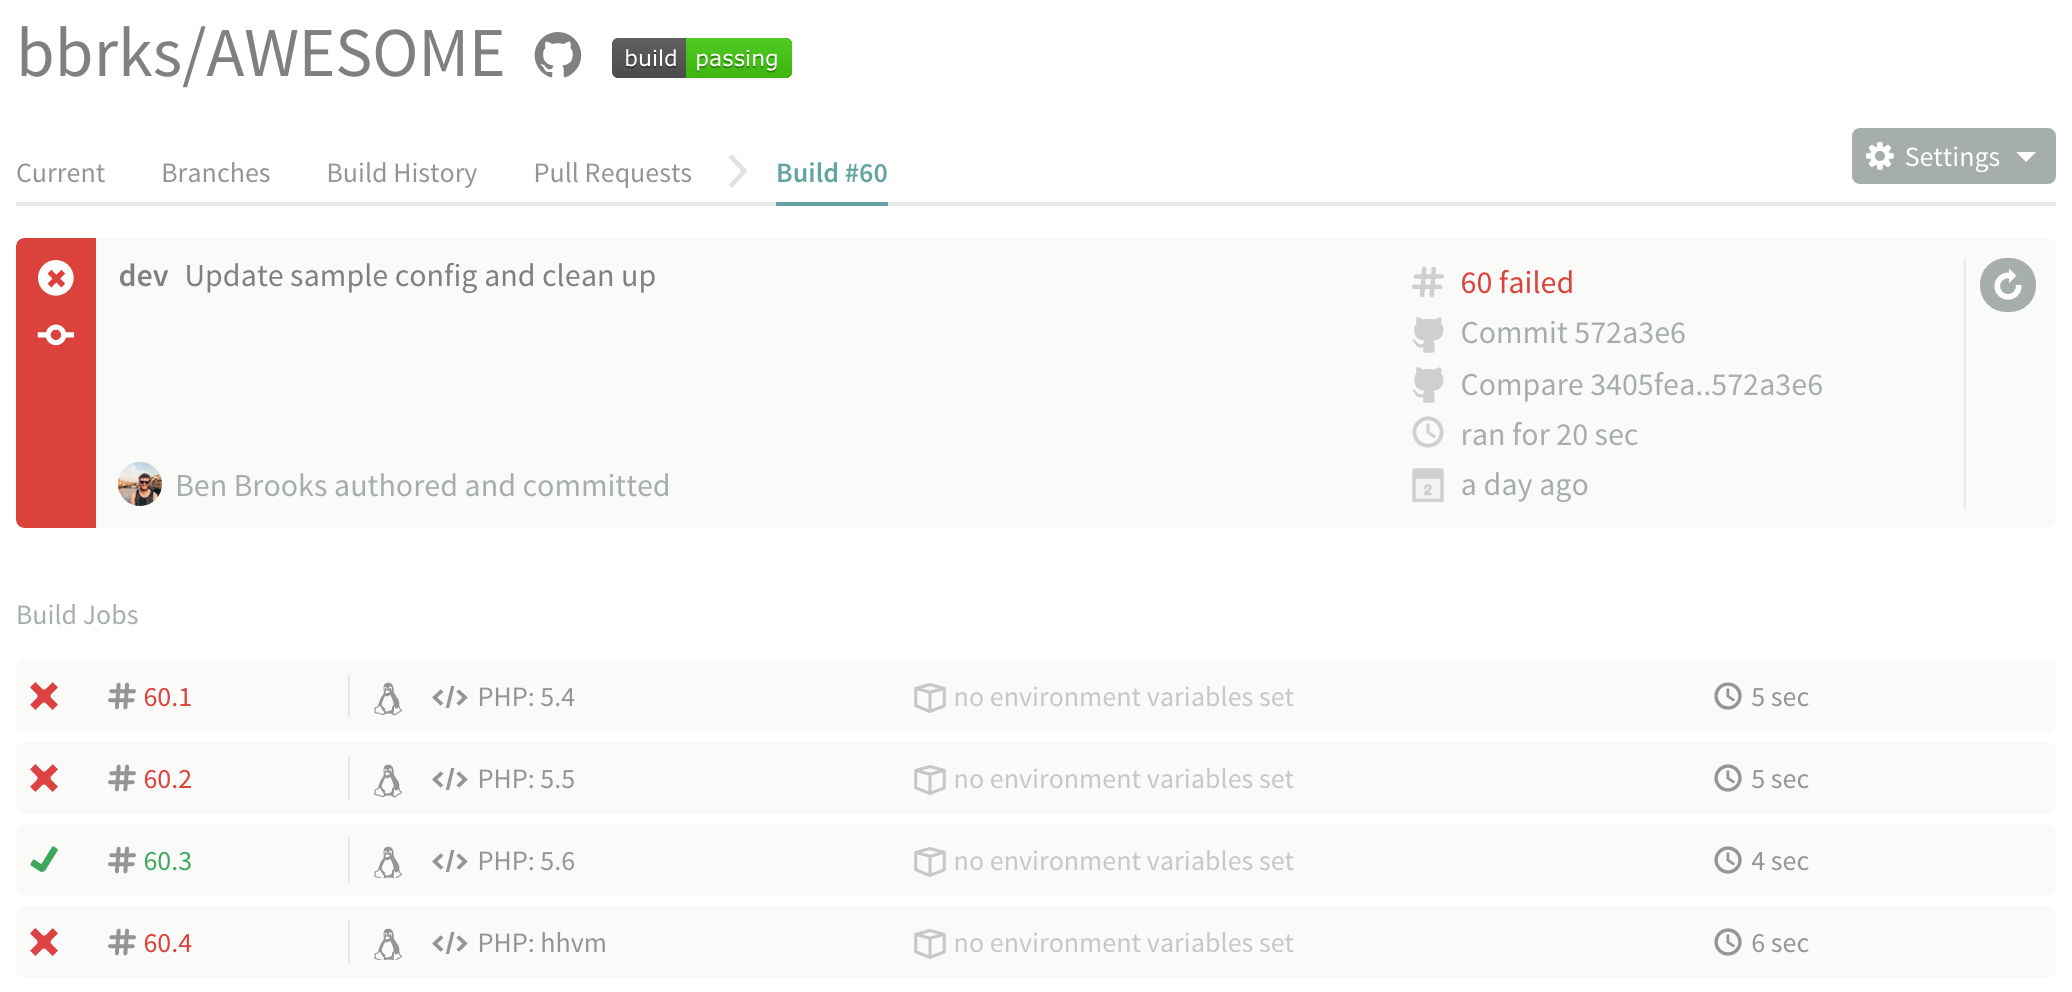
\includegraphics[width=\textwidth]{screens/travis-build}
		\caption{A screenshot of a single build in TravisCI}
		\label{fig:travisbuild}
	\end{figure}
	
	\begin{figure}[H]
		\centering 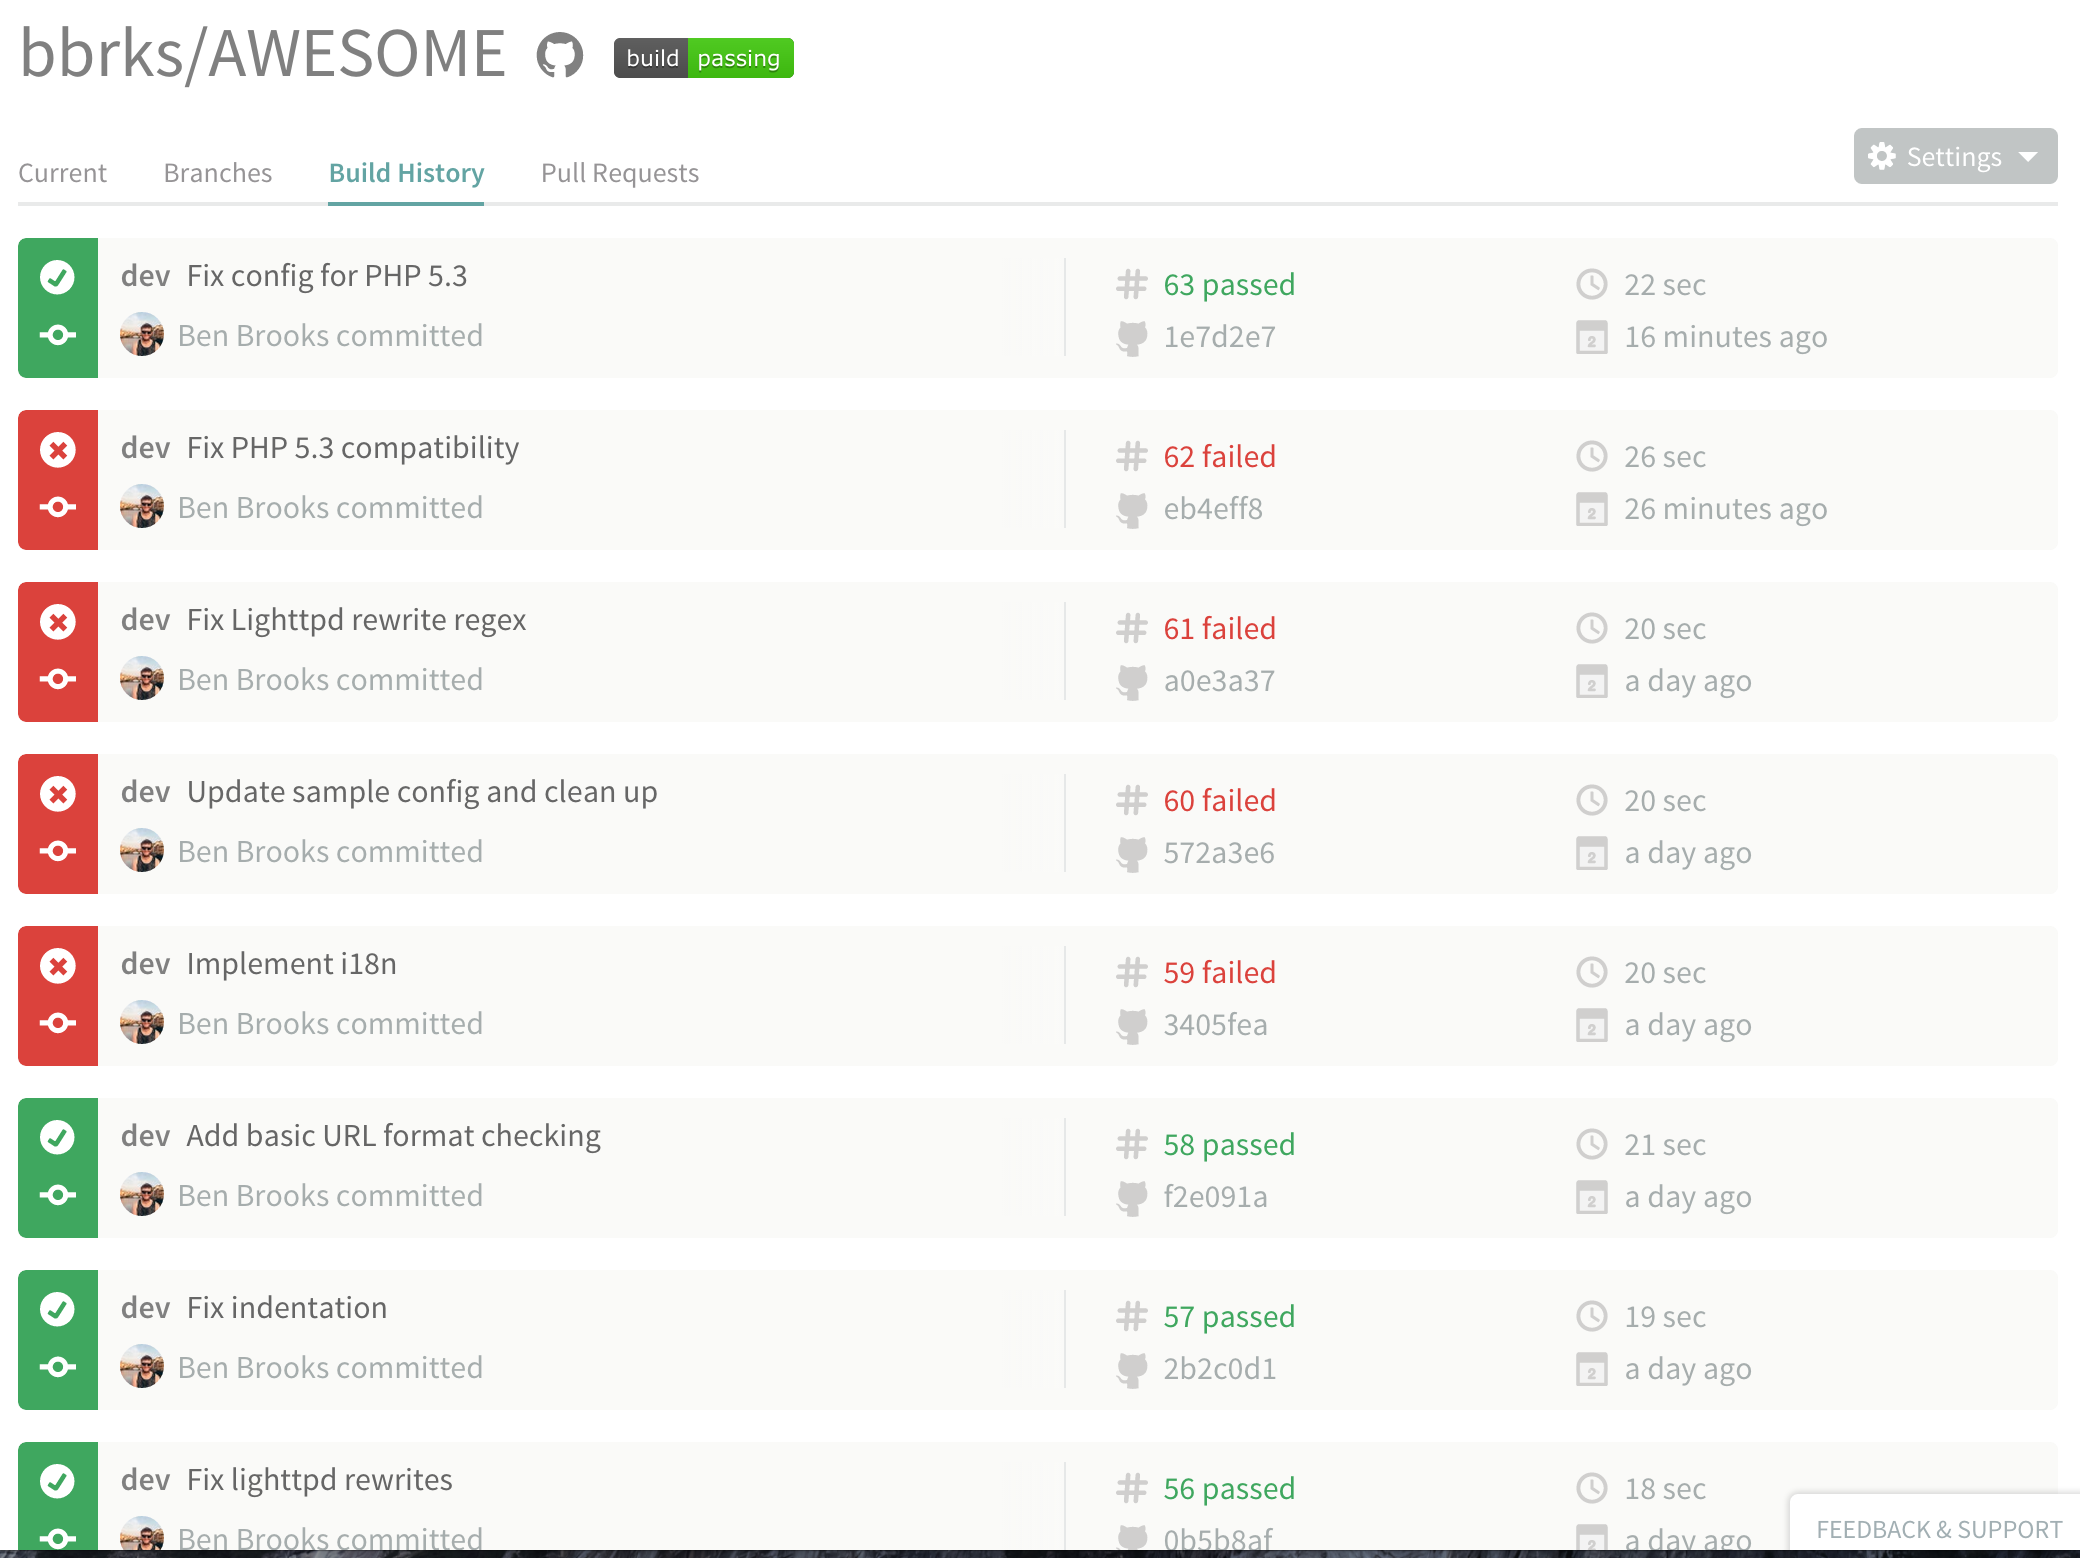
\includegraphics[width=\textwidth]{screens/travis-build-history}
		\caption{A screenshot of build history in TravisCI}
		\label{fig:travisbuildhistory}
	\end{figure}
	
	
	\subsection{Open Source License}
	\label{ssec:license}
	
	The prototype version of \ac{AWESOME} was originally under the open-source MIT license\cite{mitlicense} when branched and my work began.
	Some time after this point, the license on the original was changed to the GNU Affero General Public License, Version 3\cite{gplv3afferolicense}, however as I had branched the prototype version as it stood under the MIT license, the largely-rewritten version of \ac{AWESOME} is also licensed under the MIT license and does not touch any code licensed under the GPL v3 Affero license and so I am not restricted to using a GPL-based license.
	
	\ac{AWESOME} uses an open source, third party library for handling mail via SMTP called PHPMailer\cite{phpmailer} which is licensed under the LGPL v2 license.
	This license permits me to release \ac{AWESOME} under the MIT license without any license impositions that GPL would.
	
	Bootstrap, jQuery and jQuery StickyTabs plugin are used in the project, all of which are released under the MIT license, which again, has no restrictions on what license I have to use.
	
	\subsection{Development Environment}
	\label{ssec:devenvironment}
	
	I developed locally on my personal laptop, a MacBook Pro Retina, which ran OS X 10.10.1 at the start of this project, and now 10.10.3 at the end.
	The web server is running from Apache with PHP 5.6 via Homebrew, although later downgraded to match the PHP environment on the \ac{AU} server.
	
	Code was written in SublimeText, and most of the browser testing took place under Google Chrome and on a Nexus 5 phone.
	Git was handled through the command line, as was the compilation of \LaTeX.
	SequelPro\footnote{SequelPro Homepage: \url{http://www.sequelpro.com}} was used to connect to databases both locally and remotely.
	
	Sketch\footnote{Sketch Homepage: \url{http://bohemiancoding.com/sketch}} was used for the creation of logos and other graphics used in \ac{AWESOME}, and Dia\footnote{Dia Homepage: \url{http://dia-installer.de}} was used to create the \ac{UML} diagrams and database schema design in this report.
	
	\section{Security Audit and Code Review}
	\label{sec:securityauditimp}
	
	The security audit of \ac{AWESOME} was one of my first tasks on this project and it uncovered some issues.
	First of all, the admin login accepted any credentials, and secondly, the mysqli functions used to connect to the database are no longer recommended to be used.
	Instead, \ac{PDO} should be used to connect to databases, as this provides much better security through prepared statements, preventing SQL injection attacks.
	
	The prototype was also written in a completely procedural style, with if statements for each bit of \acl{i18n} spread throughout the codebase.
	Rewriting to use \ac{OOP} practices as well as a design pattern would kill several birds with one stone, as I could also implement \ac{PDO} and proper \ac{i18n} whilst I was at it.
	
	\section{\acl{MVC} Framework}
	\label{sec:mvcframeworkimp}
	
	The \acl{MVC} framework was fairly straight forward to code at first, especially following the tutorial mentioned previously\cite{php-mvc-tutorial}.
	However I soon ran into limitations of the framework, and the time to code in additional features ate away at the time I needed to produce a working survey tool.
	
	In the end, \ac{AU} server limitations forced me to throw away most of the functionality in the \ac{MVC} framework.
	
	\section{\acl{i18n} Framework}
	\label{sec:i18nframeworkimp}
	
	The \ac{i18n} system is small but very useful, albeit not as flexible or powerful as a mature \ac{i18n} framework.
	It has no ability to pluralise strings, nor does it offer any variable substitution like some frameworks might be expected to do.
	This lack of complexity, I think makes it better for non-technical people to provide language translations though, as everything is read in through simple JSON files.
	
	
	
	\section{Deploying to an \ac{AU} server}
	\label{sec:auserverimp}
	
	Getting \ac{AWESOME} running on a server at \ac{AU} took much longer than anticipated for a few reasons.
	Firstly, the PHP version was 5.3, which was attempted to be upgraded to 5.6, but it didn't work out, so I had to change some code to ensure it was 5.3 compatible.
	Secondly, I didn't have any direct access to the server, so any change that was made had to be zipped, sent via email to Sandy, and then he would upload the files for me, provided it was between 9am and 5pm on a weekday.
	Another issue was that the database would not connect, even though it was configured correctly.
	This was solved by Sandy adding a wildcard rule to the database hostname limit, which enabled connection from any machine.
	This poor access coupled with troubleshooting issues regarding PHP version and database connections issues were a serious hinderance.
	
	Once these issues were resolved, \ac{AWESOME} was working on the university server okay, with one condition.
	The server I was on could only be accessed through the \ac{AU} \ac{VPN}, and so anybody who received a link to a questionnaire had to either be on the university network, or connected through the university VPN to be able to view it.
	Another issue is that HTTPS was not set up correctly, and so instead of either redirecting to HTTP, or failing a certificate check, it would not allow access to \ac{AWESOME}.
	This caused problems for people using browser plugins that forced HTTPS on websites.
	
	Because of these issues, I feel that response rates through \ac{AWESOME} are significantly lower than they would otherwise be, despite being around the same 20\% figure that Google Forms had.
	
	I feel that once server access is properly fixed, response rates could be 50\% or even higher, which is a significant improvement upon previous online module evaluation methods.